\section{Solution-Aware Scoring.}

\label{sec4}

In this section, we propose {\em Solution-Aware Scoring} (SAS),
to evaluate accurately how opening a ReLU impacts the accuracy.
To do so, SAS considers explicitly a solution to a unique LP call, which is reasonably fast to obtain as there is no binary variables (polynomial time). 
%To compute $\Delta(z)$, intermediate $\Delta(b),\Delta(\hat{b})$ are computed inductively.
%Indeed, it is not rare that $z$ is sensitive to ReLU node $n$, and yet $\LP(n)$ already provides an accurate approximation of $\ReLU(n)$.
%In this case, usual heuristics would open $n$, while it would only improve the value of $z$ in a limited way.
Assume that we want to compute an upper bound for neuron $z$ on layer $\ell_z$.
We write $n < z$ if neuron $n$ is on a layer before $\ell_z$, and $n \leq z$ if $n< z$ or $n=z$. We denote ($\Sol\_\max_X^z(n))_{n \leq z}$ a solution of $\mathcal{M}_X$ maximizing $z$: $\Sol\_\max_X^z(z)$ is the maximum of $z$ under $\mathcal{M}_X$.

Consider $(\sol(n))_{n \leq z} = (\Sol\_\max_\emptyset^z(n))_{n \leq z}$, a solution maximizing the value for $z$ when all ReLU use the LP relaxation.
%(this can be obtained very efficiently by {\em one} call to an LP solver).
Function
$\Improve\_\max^z(n)=$ $\sol(z) - \Sol\_\max_{\{n\}}^z(z)$, 
accurately represents how much opening neuron $n < z$ reduces the maximum computed for $z$
compared with using only LP. 
We have $\Improve\_\max^z(n)\geq 0$ as $\Sol\_\max_{\{n\}}^z$ fulfills all the constraints of 
$\mathcal{M}_\emptyset$, so $\Sol\_\max_{\{n\}}^z(z) \leq \sol(z)$.
%Similarly, we define ($\Sol\_\min_\emptyset^z(n))_{n \leq z}$ and 
%$\Improve\_\min^z(n)$. 
Computing exactly $\Improve\_\max^z(n)$ would need a MILP call on $\mathcal{M}_{\{n\}}$ for every neuron $n \leq z$, which would be very time consuming. Instead, the SAS function uses a (single) LP call to compute $(\sol(n))_{n \leq z}$, with negligible runtime wrt the forthcoming  $\MILP_X$ call, and yet accurately approximates $\Improve\_\max^z(n)$ 
(Fig. \ref{fig_table3}).


\iffalse
That's why as far as we know, in competing heuristics to rank important nodes (e.g. \cite{BaB,huang2017safety,ferrari2022complete}), no call to solvers are made.
%Instead, we focus on the following $\Utility\_\max\nolimits^z(n)$ function upper bounding $\Improve\_\max^z(n)$. 
\fi





%\subsubsection*{Observation}

%The key of our formula is based on the following observation:



%Our observation (by experiments) is that \begin{align}
%	I_X \approx \sum_{b\in X} I_b.
%\end{align} Especially, if all neurons in $X$ are from one layer before $a$, then in %experiments, we observe that 

\iffalse
\begin{align*}
	|(I_X - \sum_{b\in X} I_b)/I_X| < 1\%. \ (\text{in experiments})
\end{align*} Even $X$ contains neurons from 3 layers before the target layer, in experiments, $I_X$ is still close to $\sum_{b\in X} I_b$.

Therefore, based on this observation, the question to choose $X$ is converted to compute $I_b$ for neurons $b$ in layers before the target layer. Our formula is to estimate the improvement of different individual neurons in different layers. For different layers, the formula will be different.  However, neither the observation in this subsection nor the formula in the next subsection has solid theoretical proof to show that they are very accurate. They are all based on experiments. 


In our algorithm, we will open neurons at most 3 layer3 before the target layer. So the formula will consists of three parts.


\subsubsection*{Compute the improvement of a single neuron}

\subsection*{One Layer before $z$}

\fi

%For all neurons $n$, let $\sol(n)=$$\Sol\_\max_\emptyset^z(n)$ be the value of neuron $a$
%in the solution of the LP instance $\Sol\_\max_\emptyset^z$ to maximize $z$.
%For one layer before the target layer, the formula is simple and most accurate. 
%To estimate $\Improve\_\max^z(a)$, 



%we define $\Utility\_\max^z(a)$, first for neurons $a$ one layer before $z$, by computing by how much the value of $z$ will change if $a$ is opened
%and other values remain the same - in particular, $value(\hat{a})=\ReLU(sol(a))$. We define:
%we first need to run $M^a_{\emptyset}$ to compute the upper bound of $a$  to obtain the solution data. Especially, we will read the values of $b$, before $\ReLU$ function and after $\ReLU$ function.

For a neuron $b$ on the layer before layer $\ell_z$, we define:


\vspace{-0.5cm}
\begin{align}
		\Utility\_\max\nolimits^z(b) = W_{bz} \times (\sol(\hat{b})- \ReLU(\sol(b)))
\end{align}
\vspace{-0.5cm}
	
	%In particular, if $\sol(\hat{a})=\ReLU(\sol(a))$, then we will have 
	%\begin{align*}
%		Utility^z(a) = 0.
%	\end{align*}


\noindent {\em Comparison:} consider $b$ with $W_{bz}<0$: 
to maximize $z$, the value of $\sol(\hat{b})$ is minimized by LP, 
ie $\sol(\hat{b})=\ReLU(\sol(b))$ thanks to Proposition~\ref{LP}. 
Thus, we have $\Utility\_\max^z(b)=0=\Improve_{max}^z(b)$.
Notice that the original scoring function $|W_{bz}|(\UB(b)-\LB(b))$ \cite{DivideAndSlide}  would be possibly very large in this case. However, {\sf GS} scoring functions from BaB-SR and FSB would also accurately compute  $s_{FSB}(b)=s_{SR}=0$.
Notice that $\Utility$ does not need to consider bias explicitly, unlike $s_{FSB},s_{SR}$,
as they are already accounted for in the solution considered. 

\medskip

Consider a neuron $a$ two layers before $\ell_z$, 
$b$ denoting neurons in the layer $\ell$ just before $\ell_z$.
Recall the rate $r(b)=\frac{\max(0,\UB(b))}{\max(0,\UB(b))-\min(0,\LB(b))} \in [0,1]$.
We define:

\newpage

\begin{flalign}
	\Delta(\hat{a}) &= \ReLU(\sol(a))-\sol(\hat{a})&&\\
	\forall b \in \ell, \Delta(b) &= W_{ab}\Delta(\hat{a})&&
\end{flalign}

\vspace{-0.6cm}

\begin{subnumcases}{\forall b \in \ell, \Delta(\hat{b}) =}
		r(b)\Delta(b), & for $W_{bz} > 0$ \\
		\max(\Delta(b),-\sol(b)), & for $W_{bz} < 0$ and $\sol(b)\geq0$\\
		\max(0,\Delta(b)+\sol(b)), & for $W_{bz} < 0$ and $\sol(b)<0$ \quad \, \quad \, \quad		 
\end{subnumcases}
\vspace{-0.4cm}
\begin{flalign}
	\Utility\_\max\nolimits^z(a) &= \Delta(z) = -\sum_{b \in \ell} W_{bz} \Delta(\hat{b})&&
\end{flalign}





\begin{figure}[t!]
	\begin{centering}
	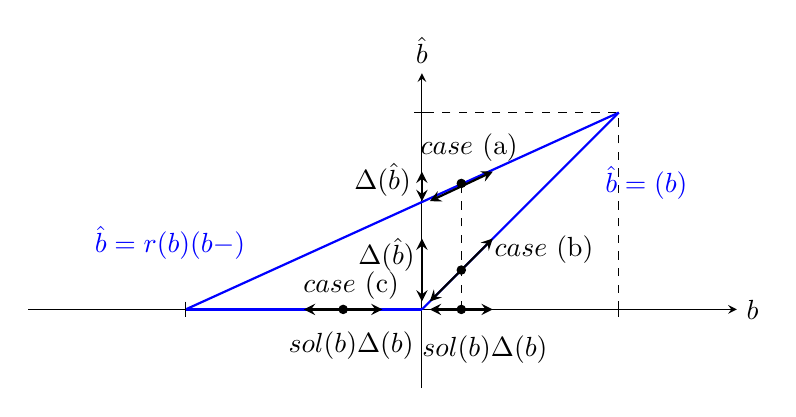
\begin{tikzpicture}[scale=1, >=stealth]
		
		% Draw axes
		\draw[->] (-5,0) -- (4,0) node[right] {$b$};
		\draw[->] (0,-1) -- (0,3) node[above] {$\hat{b}$};
		
		% Draw ReLU function
		\draw[line width=0.4mm, blue] (-3,0) -- (0,0);
		\draw[thick, blue] (0,0) -- (2.5,2.5) node[below, shift={(0.35,-0.55)}] {$\hat{b} = \ReLU(b)$};
		\draw[thick, blue] (-3,0) -- (2.5,2.5) node[above, shift={(-5.7,-2)}] {$\hat{b} = r(b) (b-\LB)$};
		
		% Add labels
		\draw[dashed] (2.5,0) -- (2.5,2.5) -- (0,2.5); % Optional grid
		\node[below left] at (0,0) {};
		
		% Add tick marks
		
		\foreach \x in {2.5}
		\draw[shift={(\x,0)}] (0,0.1) -- (0,-0.1) node[below] {$\UB$};
		\foreach \x in {-3}
		\draw[shift={(\x,0)}] (0,0.1) -- (0,-0.1) node[below] {$\LB$};
		
		\foreach \y in {2.5}
		\draw[shift={(0,\y)}] (0.1,0) -- (-0.1,0) node[left] {$\UB$};
		
		\draw[<->, thick] (0.1, 0.1) -- (0.9, 0.9) node[above,shift={(0.65,-0.45)}] {$case$ (b)}
		node[below,shift={(-0.1,-1.10)}] {$sol(b)\Delta(b)$}
		node[above,shift={(-1.35,-0.55)}] {$\Delta(\hat{b})$};
		\filldraw[black] (0.5, 0.5) circle (1.5pt);
		\filldraw[black] (0.5, 0) circle (1.5pt);
		\draw[<->, thick] (0.1, 0) -- (0.9, 0);
		\draw[dashed] (0.5,0) -- (0.5,1.6); % Optional grid
		
		
		\draw[<->, thick] (-0.5, 0) -- (-1.5, 0) node[above,shift={(0.6,0)}] {$case$ (c)}
		node[below,shift={(0.6,-0.15)}] {$sol(b)\Delta(b)$};
		\filldraw[black] (-1, 0) circle (1.5pt);
		
		
		\draw[<->, thick] (0.1, 1.375) -- (0.9, 1.75) node[above,shift={(-0.3,0)}] {$case$ (a)}
		node[above,shift={(-1.4,-0.45)}] {$\Delta(\hat{b})$};
		\filldraw[black] (0.5, 1.6) circle (1.5pt);
		
		\draw[<->, thick] (0, 0.1) -- (0, 0.9);
		
		\draw[<->, thick] (0, 1.375) -- (0, 1.75);

	\end{tikzpicture}
	\caption{Different cases for $\ReLU(b)$
%	 \vspace{-0.3cm}
}
	\label{node:b}
\end{centering}
\end{figure}

%\begin{tikzpicture}[scale=1, >=stealth]
%	
%	% Draw axes
%	\draw[->] (-5,0) -- (4,0) node[right] {$x$};
%	\draw[->] (0,-1) -- (0,3) node[above] {$y$};
%	
%	% Draw ReLU function
%	\draw[line width=0.4mm, blue] (-3,0) -- (0,0);
%	\draw[thick, blue] (0,0) -- (2.5,2.5) node[below, shift={(0.5,-0.4)}] {$y = \ReLU(x)$};
%	\draw[thick, blue] (-3,0) -- (2.5,2.5) node[above, shift={(-0.5,0.4)}] {$y = \frac{\UB}{\UB-\LB} x-\frac{\UB\LB}{\UB-\LB}$};
%	
%%	% Add labels
%%	\draw[dashed] (2,0) -- (2,2) -- (0,2); % Optional grid
%%	\node[below left] at (0,0) {$0$};
%%	
%%	% Add tick marks
%%	\foreach \x in {1,2}
%%	\draw[shift={(\x,0)}] (0,0.1) -- (0,-0.1) node[below] {\x};
%%	\foreach \y in {1,2}
%%	\draw[shift={(0,\y)}] (0.1,0) -- (-0.1,0) node[left] {\y};
%	
%\end{tikzpicture}

%We will show with a more general definition that $0 \leq \Improve\_\max^z(a) \leq \Utility\_\max^z(a)$ in Prop.~\ref{prop2}. 

%Informally, $\Delta(\hat{a}), \Delta(b), \Delta(\hat{b})$ approximate the improvement on the accuracy of $\hat{a}, b, \hat{b}$ when computing $\ReLU(a)$ using the exact MILP encoding instead of LP. 


\noindent {\em Comparison:} First, the original \cite{DivideAndSlide} does not propose a formula for node $a$ two layers before $z$. So we will compare {\sf SAS} with {\sf GS}.
Consider again the running example of Fig. \ref{img:FSB_example}. 

In the case $c\cdot d<0$, we have $\Utility\_\max\nolimits^z(a)=\Improve_{max}^z(b)=s_{FSB}(a)=s_{SR}(a)=0$, as $\Delta(\hat{a})=0$. 

In the case $c>0,d>0$, 
$\Delta(\hat{a}) = \ReLU(\sol(a))-\sol(\hat{a})$ is precise,
whereas the corresponding $\Delta_{FSB}(\hat{a}) = \LB(a) r(a)$ is only an upperbound.

The last case $c<0,d<0$ is the most extreme: 
$\Delta(\hat{b})$ adapts to the case (b),(c) in Fig. \ref{node:b} leveraging the value $\sol(b)$, which yields very different values, whereas the corresponding $\Delta_{FSB}(\hat{b})$
is always $r(b) \Delta_{FSB}(b)$: 
\begin{itemize}
\item For $sol(b)<<0$, we will have 
$\Delta(\hat{b})=0<\Delta_{FSB}(\hat{b})$.
\item For $sol(b)>>0$, we will have 
$\Delta(\hat{b})=\Delta(b) > \frac{1}{2}\Delta_{FSB}(\hat{b})$ 
as $r(b)=\frac{1}{2}$.
\end{itemize}

Further, we can show that $\Utility$ is a safe overapproximation of 
$\Improve\_\max^z(a)$, which does not hold for $s_{FSB},s_{SR}$ (because of the case $sol(b)>>0$):

\begin{proposition}
	\label{prop2}
		$0 \leq \Improve\_\max^z(a) \leq \Utility\_\max^z(a)$. 
\end{proposition}


In particular, for all nodes $a$ with $\Utility\_\max\nolimits^z(a)=0$, 
we are sure that this node is not having any impact on $\Sol\_\max_{\{a\}}^z(z)$. 
%This is one striking difference (but not the only one) with choosing utility based on 
%$|W_{az}|$ \cite{DivideAndSlide}.

	
%	
%	Similarly, let $\sol(b)$ be the value of $b$ in the LP solution of lower bound of $a$, and $\sol(\hat{b})$ be the value of $\hat{b}$. Then the formula to estimate improvement of lower bound of $b$ is: \begin{align*}
%		Improve\_min^z(b) \approx -W_{ba}(\sol(\hat{b})-\ReLU(\sol(b))).
%	\end{align*}
	
%To explain the formula, we use upper bound and the case that $W_{ba} > 0$ as an example. To compute the upper bound of $a$, $\hat{b}$ should be as large as possible. In the LP model, for fixed $\sol(b)$, the upper bound of $\hat{b}$ may be larger than $\ReLU(\sol(b))$. This is because in LP model, the upper bound of $\sol(\hat{b})$ is decided by the linear approximation rather than $\ReLU$ function. So, when neuron $b$ is open, if $\sol(b)$ do not change, then the upper bound of $a$ will be improved because the value of $\sol(\hat{b})$ will be lower to $\ReLU(\sol(b))$.
% 			
%Of course changing other variables may also effect the upper bound, but our experiments show that, the change from $\sol(\hat{b})$ to $\ReLU(\sol(b))$ is the major part of improvement. 


 



	
	\begin{proof}
    Consider $\sol'(n)_{n \leq z}$ with
	$\sol'(n)=\sol(n)$ for all $n \notin \{z,\hat{a}\} \cup \{b,\hat{b} \mid b \in \ell\}$. In particular,  $\sol'(a) = \sol(a)$.
	Now, define $\sol'(\hat{a}) = \ReLU(\sol(a))$. 
	That is, $\sol'(\hat{a})$ is the correct value for $\hat{a}$, obtained if we open neuron $a$, compared to the LP abstraction for $\sol(\hat{a})$.
	We define $\sol'(b)=\sol(b)+\Delta(b)$ and 
	$\sol'(\hat{b})=\sol(\hat{b}) + \Delta(\hat{b})$.
	Last, $\sol'(z)=\sol(z) + \sum_{b \in \ell} W_{bz} \Delta(\hat{b})$.
	We will show:
	\begin{equation}
		\label{eq12}
		(\sol'(n))_{n \leq z} \text{ satisfies the constraints in } \mathcal{M}_{\{a\}}
	\end{equation} 
	This suffices to conclude: as
	$\sol'(z)$ is a solution of $\mathcal{M}_{\{a\}}$, it is smaller or equal to the maximal solution: $\sol'(z) \leq$ $\Sol\_\max_{\{a\}}^z(z)$. That is, 
	$\sol(z)-\sol'(z) \geq \sol(z) -$ $\Sol\_\max_{\{a\}}^z(z)$, i.e. 
	$ \Utility\_\max^z(a) \geq \Improve\_\max^z(a)$.
	In particular, we have that $\Utility\_\max^z(a) \geq 0$, which was not obvious from the definition.	

Finally, we show (\ref{eq12}). First, opening $a$ changes the value of $\hat{a}$ from
	$\sol(\hat{a})$ to $\ReLU(\sol(a)) = sol(\hat{a}) + \Delta(a)$, 
	and from $sol(b)$ to $sol(b) + \Delta(b)$.
	The case of $\Delta(\hat{b})$ is the most interesting:
	If (a) $W_{bz}>0$, to maximize $z$, the LP solver sets $\sol(\hat{b})$ to the maximal possible value, which is 
	$r(b) \sol(b)+$ Cst according to Proposition \ref{LP}.
Changing $b$ by $\Delta(b)$ thus results in changing $\sol(\hat{b})$ by 
$r(b) \Delta(b)$.
If $W_{bz}\leq0$, then the LP solver sets $\sol(\hat{b})$ to the lowest possible value to maximize $z$, which happens to be $\ReLU(b)$ according to Proposition \ref{LP}.
If (b) $\sol(b) > 0$, then 
$\sol(\hat{b})=\ReLU(\sol(b))=\sol(b)$, and the change to $\hat{b}$ will be 
the full $\Delta(b)$, unless $\Delta(b) < -\sol(b) < 0$ in which case it is 
$-\sol(b)$.
If (c) $\sol(b) < 0$, then we have $\sol(\hat{b})=\ReLU(b)=0$ and opening $a$ moves away 
from 0 only if $\sol(b)+\Delta(b)>0$. 
\qed
\end{proof}


\iffalse

	If we open $a$ without changing its value $\sol(a)$, then the change $\Delta(\hat{a})$ in the weight of $\hat{a}$ is 
$\Delta(\hat{a})=\ReLU(\sol(a)) - \sol(\hat{a}) \leq 0$ as above. Its impact on $z$ is no more direct with $W_{az}$, but it is through $\ell$. 
We let $\Delta(b) = W_{ab}\Delta(\hat{a})$ for all $b \in \ell$.
Based on Proposition \ref{LP}, we can evaluate the impact 
$\Delta(\hat{b})$ of opening $a$ on the value of each $\hat{b}$, by using the upper and lower bound $\UB(b),\LB(b)$:

	\begin{align*}
		&\Delta(\hat{b}) =
		\begin{cases}
			\frac{\UB(b)}{\UB(b)-\LB(b)}\Delta(b),  &\text{if }W_{bz} > 0\\
			\max(\Delta(b),-\sol(b)),  &\text{if }  W_{bz} < 0 \text{ and } \sol(b)\geq0\\
			\max(\Delta(b)+\sol(b),0),  &\text{if }  W_{bz} < 0 \text{ and } \sol(b)<0		 
		\end{cases}
		\end{align*}


Indeed, if $W_{bz}>0$, then according to Proposition \ref{LP}, the LP solver
sets $\sol(\hat{b}) = \sol(b) \frac{\UB(b)}{\UB(b)-\LB(b)} +$ Cst to maximize $z$.
Changing $b$ by $\Delta(b)$ thus results in changing $\sol(\hat{b})$ by 
$\frac{\UB(b)}{\UB(b)-\LB(b)}\Delta(b)$.
If $W_{bz}\leq0$, then the LP solver sets $\sol(\hat{b})$ to the lowest possible value to maximize $z$, which happens to be $\ReLU(b)$ according to Proposition \ref{LP}.
If $\sol(b) < 0$, then we have $\sol(\hat{b})=\ReLU(b)=0$ and opening $a$ change the 0 value only if $\sol(b)+\Delta(b)>0$. If $\sol(b) > 0$, then 
$\sol(\hat{b})=\ReLU(\sol(b))=\sol(b)$, and the change to $\hat{b}$ will be 
the full $\Delta(b)$, unless $\Delta(b) < -\sol(b) < 0$ in which case it is 
$-\sol(b)$. We then set:

%We then define 
%\begin{align*}
%	Utility\_max^z(a) = (\sol(\hat{a})-\ReLU(\sol(a)))\sum_b k(b).
%\end{align*}

$$ \Utility\_\max\nolimits^z(a) = -\sum_{b \in \ell} W_{bz} \Delta(\hat{b})$$
\fi

%We proceed inductively to define $\Utility\_\max^z(a)$ for deeper neurons $a$.

\iffalse
While $\Utility$ is a priori a more accurate way to select neurons to open in partial MILP (that will be verified in Fig. \ref{fig_table3}), global scoring functions have two advantages: first, they are faster to compute (a unique backpropagation is sufficient, while SAS needs one LP call to recover the solution, plus a forward propagation for each node $a$). This is not an issue for selecting nodes for partial MILP, as there is a single selection step. This would be potentially problematic for choosing branching nodes in BaB, at each branch. A trade off could be to precompute FSB and only on the most promising nodes run $\Utility$. The second shortcoming is the other side of the coin to consider improvement local to a solution: in the case of branching, one of the branch imposes to be far from the solution and $\Utility$ is not accurate on that branch, while global scoring is as (in)accurate for both branches. We will verify that using GS for ordering nodes after the SAS selection is actually more efficient, for this very reason.
\fi

%\textcolor{red}{$s_{FSB}$ *is* in Figure 5, under label “GS” (global-scoring). $s_{SR}$ is very slightly worst, reason why we did not report it.}

\iffalse
We use the following formula for general cases, i.e. possibly more than 3 layers. We use $a$ to denote the source node, and use $b,c$ to denote that $b$ is in one layer before $c$. 

\begin{align*}
	\Delta(\hat{a}) &= \ReLU(\sol(a))-\sol(\hat{a})\\
	\Delta_0(b) &= \sum_{b} W_{bc}\Delta(\hat{b})\\
		\Delta(c) &= \min(\max((\sol(c)+\Delta_0(c),\LB(c))),\UB(c))-\sol(c)\\
		\Delta(\hat{c}) &=
		\begin{cases}
		\Delta(c)\frac{\LB(c) - \sol(\hat{c})}{\LB(c) - \sol(c)},  &\text{if } \LB(c)< \sol(c) < 0\\
		\Delta(c)\frac{\UB(c) - \sol(\hat{c})}{\UB(c) - \sol(c)},  &\text{if }  0< \sol(c) < \UB(c)\\
			\Delta(c),  &\text{else } 	 
		\end{cases}
\end{align*}


\subsubsection*{Three Layer before  $z$} 

Suppose $a$ is a neuron in three layers before $z$, we use $b$ to denote neurons in two layer before $z$ and $c$ to denote neurons in one layer before $z$ and. 

This formula is based on previous subsection but more complex. In some network, running this formula may cost too much time. 

The key problem is how to compute the coefficient $k$ for neurons in two layers before the target layer. To do this, we may use the values in the solution of LP model as follows:

\begin{definition}\label{3layer}
Let $\UB$ and $\LB$ denote the precomputed upper bounds and lower bounds used in building MILP models. We define the following function $h$ for all neurons $b$ in two layers before the target neuron $z$ as follows:
	\begin{align}
		&v_0 = \sol(\hat{b}), v_1 = \ReLU(\sol(b)), v_2 = \frac{\UB(b)\sol(b)-\UB(b)\LB(b)}{\UB(b)-\LB(b)}\\
		&h(b) =
		\begin{cases}
			\frac{v_0-v_1}{v_2-v_1}, & \text{if } v_2-v_1 > 0\\
			0.5, & \text{otherwise.}
		\end{cases}
	\end{align} 
\end{definition} 

\begin{definition}
	Continue the assumption in Definition \ref{3layer}. We define function $D$ layer by layer.
	
	First, $\Delta(a) = \ReLU(\sol(a))-\sol(\hat{a})$.
	
To compute $\Delta(b)$ for neurons $b$ in two layer before $z$, we define \begin{align}
	&u_0 = \max(\LB(b),\min(\UB(b),  \sol(b)+\Delta(a)W_{ab}))\\
	&u_1 = \begin{cases}
		\ReLU(u_0)+h(b)(\frac{\UB(c)u_0-\UB(b)\LB(b)}{\UB(b)-\LB(b)}-\ReLU(u_0)), & \text{if }\LB(b) < 0\\
	u_0, & \text{if }  \LB(b) \geq 0
	\end{cases}\\
	&\Delta(b) = u_1-\sol(\hat{b})
\end{align}
	
	To compute $\Delta(c)$ for neurons $c$ in one layer before $z$, we define 
	\begin{align}
		&w_0 = \sum_b \Delta(b)W_{bc}\\
		&w_1 = \min(\UB(c),\sol(c)+w_0)\\		
		&\Delta(c) =
		\begin{cases}
			w_1-\sol({c}), & \text{if }W_{cz} > 0 \text{ and } \LB(c)\geq 0\\
		k(c)(w_1-\sol({c})), & \text{if }W_{cz} > 0 \text{ and } \LB(c)< 0\\
		\ReLU(w_1)-\sol(\hat{c})	, & \text{if }  W_{cz} < 0
		\end{cases}\\
		&\Delta(z) = \sum_c \Delta(c)W_{cz}\\
		&\Utility\_\max^z(a) = -\Delta(z)
	\end{align}
\end{definition}
		
\fi